%------------------------------------------------
%     THEMES
%------------------------------------------------

\documentclass[10pt]{beamer}
\usefonttheme{professionalfonts} % using non standard fonts for beamer

\setbeamersize{text margin left=30mm,text margin right=30mm} 

\usetheme{Wisconsin}


\usepackage{graphicx}
\usepackage{tabularx}
\usepackage{array}
\usepackage{bm}
\usepackage[most]{tcolorbox}
\usepackage{mathtools}
\usepackage{stackengine}
\usepackage{algorithmic}
\usepackage{epstopdf}
\usepackage{lipsum}

\newcommand\blfootnote[1]{%
  \begingroup
  \renewcommand\thefootnote{}\footnote{#1}%
  \addtocounter{footnote}{-1}%
  \endgroup
}



%% Colors
\definecolor{forestgreen}{rgb}{0.13, 0.55, 0.13}
\definecolor{green2}{rgb}{0, 0.8, 0}
\definecolor{UWGray}{RGB}{90,90,90}
\definecolor{UWRed}{RGB}{183,1,0}
\setbeamerfont{block title}{size={}}
\setbeamercolor{block title}{fg=UWRed}

\newcommand{\red}{\color{red}}
\newcommand{\blue}{\color{blue}}
\newcommand{\green}{\color{green2}}
\newcommand{\UWgray}{\color{UWGray}}
\newcommand{\UWred}{\color{UWRed}}
\graphicspath{{../figs/}}
%% \graphicspath{{../../FIGS/old_figs/}}               

%% Beamer macros
\newcommand{\backupbegin}{
   \newcounter{finalframe}
   \setcounter{finalframe}{\value{framenumber}}
}
\newcommand{\backupend}{
   \setcounter{framenumber}{\value{finalframe}}
}

%% Sungho Macros
\newcommand{\bx}{\mathbf{x}}
\newcommand{\bX}{\mathbf{X}}
\newcommand{\bW}{\mathbf{W}}
\newcommand{\bw}{\mathbf{w}}
\newcommand{\bbeta}{\mathbf{\beta}}
\newcommand{\bepsilon}{\mathbf{\epsilon}}
\newcommand{\bPhi}{\boldsymbol{\Phi}}
\newcommand{\bphi}{\boldsymbol{\phi}}
\newcommand{\bLambda}{\mathbf{\Lambda}}
\newcommand{\blambda}{\mathbf{\Lambda}}
\newcommand{\bt}{\mathbf{t}}
\newcommand{\bht}{\hat{\mathbf{t}}}
\newcommand{\bp}{\mathbf{p}}
\newcommand{\bY}{\mathbf{Y}}
\newcommand{\bZ}{\mathbf{Z}}
\newcommand{\by}{\mathbf{y}}
\newcommand{\bC}{\mathbf{C}}
\newcommand{\bc}{\mathbf{c}}
\newcommand{\bd}{\mathbf{d}}
\newcommand{\bA}{\mathbf{A}}
\newcommand{\ba}{\mathbf{a}}
\newcommand{\bB}{\mathbf{B}}
\newcommand{\bb}{\mathbf{b}}
\newcommand{\bK}{\mathbf{K}}
\newcommand{\bH}{\mathbf{H}}
\newcommand{\bG}{\mathbf{G}}
\newcommand{\bI}{\mathbf{I}}
\newcommand{\bS}{\mathbf{\Sigma}}
\newcommand{\bR}{\mathbf{R}}
\newcommand{\br}{\mathbf{r}}
\newcommand{\bs}{\mathbf{s}}
\newcommand{\bu}{\mathbf{u}}
\newcommand{\bU}{\mathbf{U}}
\newcommand{\bP}{\mathbf{P}}
\newcommand{\bv}{\mathbf{v}}
\newcommand{\bV}{\mathbf{V}}
\newcommand{\bg}{\mathbf{g}}
\newcommand{\bh}{\mathbf{h}}
\newcommand{\bq}{\mathbf{q}}
\newcommand{\bQ}{\mathbf{Q}}
\newcommand{\bxi}{\boldsymbol{{\xi}}}
\newcommand{\bup}{\boldsymbol{\upsilon}}
\newcommand{\rank}{\mathop{\textrm{\textup{rank}}}}
\newcommand{\diag}{\mathop{\textrm{\textup{diag}}}}
\newcommand{\st}{\mathop{\textrm{\textup{s.t.}}}}
\newtheorem{proposition}{Proposition}

\usepackage{media9}
\usepackage{movie15}
\usepackage{animate}
%% \newcommand{\includemovie}[3]{%
%% \includemedia[%
%% width=#1,height=#2,%
%% activate=pagevisible,%
%% deactivate=pageclose,%
%% addresource=#3,%
%% flashvars={%
%% src=#3 % same path as in addresource!
%% &autoPlay=true % default: false; if =true, automatically starts playback after activation (see option ‘activation)’
%% &loop=true % if loop=true, media is played in a loop
%% &controlBarAutoHideTimeout=0 %  time span before auto-hide
%% }%
%% ]{}{StrobeMediaPlayback.swf}%
%% }% end of the new command


%-----------------------------------------------------------
%    TITLE PAGE
%-----------------------------------------------------------

\title{\LARGE Low-Rank System Identification for \\High-Dimensional Spatio-Temporal Data}
\author{Sungho Shin and Victor M. Zavala} 
\institute[UW-Madison] 
{\small
  Department of Chemical and Biological Engineering\\
  University of Wisconsin-Madison\\
\medskip
\textit{sungho.shin@wisc.edu; victor.zavala@wisc.edu}
}
\date{MLSE 2019, Atlanta} 

\begin{document}

\begin{frame}
  \titlepage
\end{frame}

%------------------------------------------------
\begin{frame}{Spatio-temporal data}
  \begin{columns}
    \begin{column}{0.55\textwidth}
      \begin{itemize}
      \item Spatio-temporal phenomena are pervasive in science and engineering.
        \vspace{0.2in}
      \item Analysis of spatio-temporal data is becoming increasinlgy important.
        \vspace{0.2in}
      \item Analysis is difficult due to {\red high dimensionality} and {\red absence of physics-based models}.
        \vspace{0.2in}
      \item Want to develop scalable {\blue system identification} tools.
      \end{itemize}
    \end{column}
    \begin{column}{0.45\textwidth}
      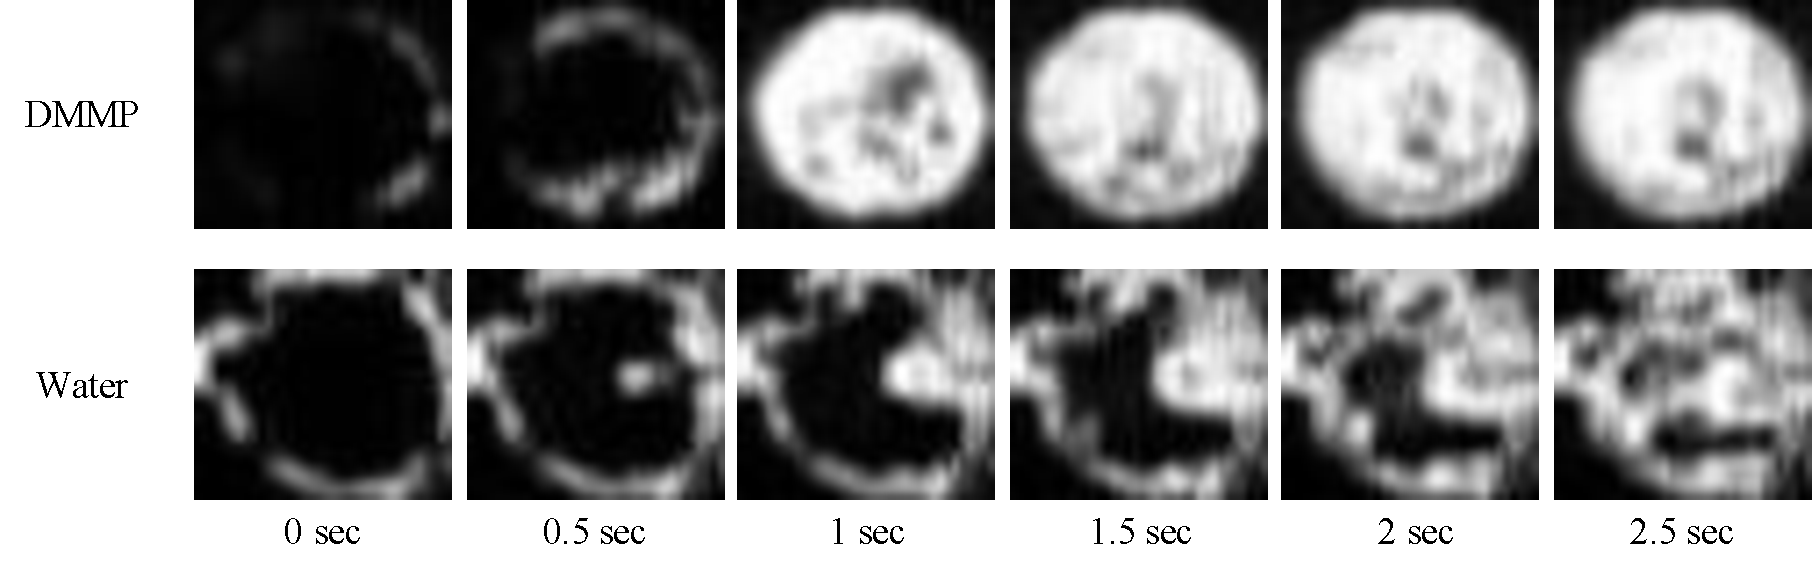
\includegraphics[width=\textwidth]{../fig/lc-raw.pdf}\\
      \vspace{0.2in}
      \includegraphics[width=\textwidth]{../fig/elec-raw.pdf}
      %% \vspace{0.1in}
      %% \includegraphics[width=\textwidth]{../fig/flow-example.jpg}\\
    \end{column}
  \end{columns}
  \blfootnote{Image source: Shao et al. (2019)}
\end{frame}
%------------------------------------------------

%------------------------------------------------
\begin{frame}{Linear system identification (ID)}
    \begin{block}{Problem}
      Consider fitting dynamic model $\bx^+ = \bA\bx$ to data $\{\bx_1,\cdots,\bx_{n+1}\in\mathbb{R}^m\}$. The system ID problem can be posed as:
      \begin{align*}
      \min_{\bA\in\mathbb{R}^{m\times m}} \Vert \bY - \bA \bX \Vert_F^2,
      \end{align*}
      where the data matrices are defined as $\bX :=
      \begin{bmatrix}
        \bx_1 \cdots \bx_n
      \end{bmatrix}$, $
      \bY :=
      \begin{bmatrix}
        \bx_2 \cdots \bx_{n+1}
      \end{bmatrix}$.
    \end{block}
    \begin{itemize}
    \item $\Vert\mathbf{M}\Vert_F:=\left(\sum_{i,j}{(m_{ij}})^2 \right)^{1/2}$ is the Frobenius norm.
      \vspace{0.1in}
    \item Solution can be computed using economy-sized SVD of $\bX=\bU\bS\bV^\top$ as:
      \begin{align*}
        \blue \bA= \bY\underbrace{\bV \bS^{-1} \bU^\top}_{\bX^\dag}.
      \end{align*}
    \item This is a data-driven \& black-box ID method.
    \end{itemize}
\end{frame}
%------------------------------------------------

%------------------------------------------------
\begin{frame}{Challenges of system ID}
  
  \begin{columns}
    \begin{column}{0.5\textwidth}
      \begin{itemize}
      \item $\bA$ is { high-dimensional, unstructured (dense), and hard to interpret} (e.g., ${10^4\times 10^4}$).
        \vspace{0.2in}
      \item High memory requirements: \\
        (e.g., $10^8$ data entries, $\sim 1$ GB)
        \vspace{0.2in}
      \item Using $\mathbf{A}$ for simulation or optimization is expensive.
              \vspace{0.2in}
    \item \red Conventional system ID is not effective for spatio-temporal data.
      \end{itemize}
    \end{column}
    \begin{column}{0.45\textwidth}
      \includegraphics[width=\textwidth]{../fig/spatiotemporal.pdf}\\
      \vspace{0.1in}
      Spatial dimension $m\approx 10^4$, \\
      Temporal dimension $n\approx 10^2$
    \end{column}
  \end{columns}
  %% \vspace{0.2in}
  %% {\UWred We aim to develop a strategy to overcome the shortcomings of conventional system ID.}
\end{frame}
%------------------------------------------------

%------------------------------------------------
\begin{frame}{Identification of low-rank dynamic mapping}
  \begin{block}{Problem}
    \vspace{-0.15in}
    \begin{align*}
      \min_{\bA\in\mathbb{R}^{m\times p}}\;& \Vert \bY - \bA \bX \Vert_F^2\\
      \st\;&{\blue \rank(\bA)\leq r.}
    \end{align*}
  \end{block}
  %% \begin{block}{Problem}
  %%   \vspace{-0.2in}
  %%   \begin{align*}
  %%     \min_{\bA\in\mathbb{R}^{m\times m}}\;& \Vert \bY - \bA \bX \Vert_F^2\\
  %%     \st\;&{\blue \rank(\bA)\leq r.}
  %%   \end{align*}
  %% \end{block}
  \begin{itemize}
  \item Induce low-complexity {\blue structure}: $\bA=\bP\bQ^\top$ ($\bP\in\mathbb{R}^{m\times r}$ and $\bQ\in\mathbb{R}^{m\times r}$).
    \begin{center}\includegraphics[width=.5\textwidth]{../fig/PQ.pdf}\end{center}
  \item {\blue More interpretable model}. 
    \vspace{0.1in}
  \item {\blue Reduce memory and enable efficient computation}.
    \vspace{0.1in}
  \item[x] Rank-constraints are {\red difficult to handle}.
  \end{itemize}
\end{frame}
%------------------------------------------------

\section{Dynamic mode decomposition (state-of-the-art technique)}
%------------------------------------------------
\begin{frame}{Outline}
  \tableofcontents[currentsection]
\end{frame}
%------------------------------------------------

%------------------------------------------------
\begin{frame}{Singular value decomposition (SVD)}
  \begin{block}{Theorem}
    There exists {\blue\em economy-sized SVD} of $\bX \in \mathbb{R}^{m\times n }$:
    \begin{align*}
      \bX = \bU \bS \bV^\top
    \end{align*}
    \vspace{-0.2in}
    \begin{itemize}
    \item[\textcolor{black}{\textbullet}]
      %% $\bS = \begin{bmatrix} \sigma_1\\&\ddots\\ &&\sigma_\ell\end{bmatrix}$
      $\bS = \diag(\sigma_1,\cdots,\sigma_\ell)$
      with $\sigma_1\geq \cdots\geq \sigma_\ell>0$.
    \item[\textcolor{black}{\textbullet}] $\bU\in\mathbb{R}^{m\times \ell}$, $\bV\in\mathbb{R}^{n\times \ell}$ are orthogonal
    \item[\textcolor{black}{\textbullet}] $\ell=\rank(\bX)$ 
    \end{itemize}
  \end{block}
 % \begin{center}
   % \includegraphics[width=.6\textwidth]{../fig/SVD.pdf}
  %\end{center}
  \vspace{0.1in}
  \begin{itemize}
\item SVD provides mechanism to compute low-rank approximations for matrices.
  \vspace{0.1in}
  \item {\em\blue Rank-$r$ truncated svd}: rank-$r$ approximation of $\mathbf{X}$ can be obtained by taking the $r$ largest singular values.
    \begin{align*}
      \bX\approx \bX_{(r)}=\bU_{(r)}\bS_{(r)}\bV_{(r)},
    \end{align*}
    where $\bS_{(r)} := \bS(1:r,1:r)$, $\bU_{(r)} := \bU(:,1:r)$, and $\bV_{(r)} := \bV(:,1:r)$.
  \end{itemize}
\end{frame}
%------------------------------------------------

%------------------------------------------------
\begin{frame}{Low-rank matrix approximation}
      \begin{theorem}[Eckart-Young-Mirsky]
        Consider data $\bX\in\mathbb{R}^{m\times n}$ and the following problem
          \begin{align*}
            \min_{\bX'\in\mathbb{R}^{m\times n}}\; &\Vert \bX'-\bX\Vert^2_F\\
            \st\;& \rank(\bX')\leq r.
          \end{align*}
          Solution is rank-$r$ truncated SVD of $\bX$:
          \begin{align*}
            \blue\bX_{(r)} = \bU_{(r)}\bS_{(r)}(\bV_{(r)})^\top.
          \end{align*}
      \end{theorem}
      \begin{itemize}
      \item Applications: image compression, feature extraction, matrix completion, {\blue model reduction}, etc.
      \end{itemize}
      \begin{center}
        \includegraphics[width=.34\textwidth]{../fig/compression.pdf}
%        \includegraphics[width=.18\textwidth]{../fig/pca.pdf}
        \includegraphics[width=.33\textwidth]{../fig/movie.pdf}
      \end{center}
\end{frame}
%------------------------------------------------



%------------------------------------------------

%------------------------------------------------
\begin{frame}{Dynamic mode decomposition {\small (DMD, state-of-the-art)}}
  \begin{block}{Problem (Schmid 2010, {\em J. of fluid mechanics})}
    \vspace{-0.1in}
    \begin{align*}
      \min_{\bA\in\mathbb{R}^{m\times m}} \Vert \bY - \bA {\blue \bX_{(r)}} \Vert_F^2,
    \end{align*}
  \end{block}
  \begin{itemize}
  \item DMD uses {\blue rank-$r$ approximation $ \bX_{(r)}=\bU_{(r)}\bS_{(r)}\bV_{(r)}^\top$} of $\bX$.
    \vspace{0.15in}
  \item The solution can be computed by
    \begin{align*}
      \bA = \bY \underbrace{\bV_{(r)}(\bS_{(r)})^{-1}(\bU_{(r)})^\top}_{(\bX_{(r)})^\dag}
    \end{align*}
  \item Rank constraint $\blue \rank(\bA)\leq r$ is indirectly enforced.
    \vspace{0.15in}
 % \item Computational complexity is $O(r^2\max(m,n))$.\\
   % (the solution for $m\sim 10^4$ and $n\sim 10^2$ data can be found in $\sim 0.1$ secs).
  \item Matrix $\mathbf{A}$ encodes spatio-temporal behavior of the system.
    %% \item[x] The sequential strategy may deliver significantly suboptimal solution
    \begin{center}
      \includegraphics[width=.7\textwidth]{../fig/dm-schematic-3.pdf}\\
      {\em\blue dynamic modes}
    \end{center}
  \end{itemize}
\end{frame}
%------------------------------------------------

%------------------------------------------------
\begin{frame}{Spatio-temporal evolution}
  \begin{block}{Proposition}
  %% Assuming $\bI-\bA$ is nonsingular, with $\overline{\bx}:=(\bI-\bA)^{-1}\bB\overline{\bu}$, rewrite the system as:
  %% \begin{align*}
  %%   \bx^+-\bx_0 = \bA(\bx-\bx_0).
  %% \end{align*}
  The evolution of $\bx^+ = \bA \bx $ can be written as expansion:
  \begin{align*}
    \bx(t) = \sum_{j=1}^r b_j{\red (\lambda_j)^{t/\Delta t}}{\blue \bphi_j},\quad t\in\mathbb{R}_{\geq 0}
  \end{align*}
  where $(\lambda_j,\bphi_j)$ are the eigenpairs of $\bA$.
  \end{block}
  \begin{itemize}    
  \item We call {\blue $\bphi_j\in\mathbb{C}^{m}$ a {\em spatial mode}} and {\red $\lambda_j\in\mathbb{C}$ a {\em temporal mode}}.
    \vspace{0.05in}
    \begin{center}
      \includegraphics[width=.8\textwidth]{../fig/dm-schematic-2.pdf}
    \end{center}
  %% \item We call {\blue $\overline{\bx}\in\mathbb{R}^{m}$ a {\em stationary mode}}. 
    %%   \vspace{0.1in}
  \item Dynamic modes $(\lambda_j,\bphi_j)$  provide information on spatial and temporal scales.
    \vspace{0.1in}
  \item Number of dynamic modes = {\blue\em $\rank(\bA)$}.
    \vspace{0.1in}
  \item Low-rankness in $\bA$ enables a {\blue concise representation of dynamics}.
  %%   \vspace{0.1in}
  %% \item Low-rankness enables concise representation of dynamic modes.
    %% \vspace{0.1in}
    %% \begin{block}{}\bf\centering
    %%   Eigenvectors and eigenvalues are important information that can charactrize the dynamics    \end{block}
  \end{itemize}
\end{frame}
%------------------------------------------------
%------------------------------------------------
\begin{frame}{Dynamic mode extraction}
  \centering
  \begin{tikzpicture}[thick,scale=0.75, every node/.style={transform shape}]
    \node[anchor=north west] at (-2.8,8) {Spatio-temporal data};
    \node[anchor=north west] at (3.3,8) {Low-rank model};
    \node[anchor=north west] at (9.2,8) {Dynamic modes};
    \fill[black,opacity=0.2,rounded corners] (-2.8,5) rectangle (.8,8);
    \fill[black,opacity=0.2,rounded corners] (3.3,5) rectangle (6.8,8);
    \fill[black,opacity=0.2,rounded corners] (9.2,5) rectangle (12.8,8);
    \node at (-1.8,6.25) [draw,thick,minimum width=1cm,minimum height=1.5cm] {$\bX$};
    \node at (-0.2,6.25) [draw,thick,minimum width=1cm,minimum height=1.5cm] {$\bY$};
    %% \node at (4,6.25) {$\mathcal{A}=$};
    \node at (5.2,6.25) {$=$};
    \node at (6.7,6.8) {$\top$};
    \node at (4.2,6.25) [draw,thick,minimum width=1.5cm,minimum height=1.5cm] {$\bA$};
    \node at (5.7,6.25) [draw,thick,minimum width=.2cm,minimum height=1.5cm] {$\bP$};
    \node at (6.2,6.25) [draw,thick,minimum width=.2cm,minimum height=1.5cm] {$\bQ$};
    %% \node at (6.2,6.25) [draw,thick,minimum width=1cm,minimum height=1cm] {$\bB$};
    \node at (11,7) {$\bPhi=\begin{bmatrix}\bphi_1&\cdots&\bphi_r\end{bmatrix}$ };
    \node at (11,6) {$\bLambda=\begin{bmatrix}\lambda_1\\&\ddots\\&&\lambda_r\end{bmatrix}$ };
    \draw[->] (0.9,6.5) -- (3.1,6.5);
    %% \node (rect) at (2,7) {
    %%   \begin{tabular}{cc} Low-rank \\System ID
    %% \end{tabular}};
    \draw[->] (6.9,6.5) -- (9.1,6.5);
    %% \node (rect) at (8,7) {
    %%   \begin{tabular}{cc} Dynamic mode \\extraction\end{tabular}};
  \end{tikzpicture}
  \vspace{0.2in}
  \begin{itemize}
  \item Dynamic modes obtained by eigendecomposition of $\tilde{\bA}:=\bQ^\top \bP\in\mathbb{R}^{r\times r}$ {\blue }:
    \begin{align*}
      \tilde{\bA} \tilde{\bPhi}&= \tilde{\bPhi} \bLambda \;\Rightarrow\; \bA \underbrace{\bP\tilde{\bPhi}}_{\bPhi} = \underbrace{\bP\tilde{\bPhi}}_{\bPhi}\bLambda      
    \end{align*}
    (Tu et al. 2014)
    \vspace{0.1in}
  \item {\blue Computation is not expensive.}
  \end{itemize}
\end{frame}
%------------------------------------------------
%------------------------------------------------
\begin{frame}{Illustrative example (diffusion)}
  \begin{block}{Example}
    Consider {\blue data} obtained from simulation of:
    \begin{align*}
      \frac{\partial}{\partial t} {x}(t,z) &= k\frac{\partial^2}{\partial z^2} {x}(t,z)\tag{diffusion equation}\\
      {x}(0,z)&=\bar{{x}}(z)\tag{initial condition}\\
      {x}(t,0)&={x}(t,1)=0\tag{boundary condition}
    \end{align*}
  \end{block}
  \centering
  
  \includegraphics[width=.9\textwidth]{../fig/diff-raw.pdf}
\end{frame}
%------------------------------------------------

%------------------------------------------------
\begin{frame}{Visualization of dynamic modes}
  \begin{center}
    \includegraphics[width=.8\textwidth]{../fig/diff-3.pdf}
  \end{center}
  \begin{itemize}
  \item Rank-3 solution obtained.
    \vspace{0.1in}
  \item Observe that the higher the spatial frequency the faster decay.
    \vspace{0.1in}
  \end{itemize}
\end{frame}
%------------------------------------------------


\section{Low-rank system identification (our contribution)}
\begin{frame}{Outline}
\tableofcontents[currentsection]
\end{frame}
%------------------------------------------------
\begin{frame}{Low-rank system ID: formulation}
  \begin{block}{Problem}
    Consider $\bX\in\mathbb{R}^{p\times n}$ and $\bY\in\mathbb{R}^{m\times n}$. Low-rank system ID problem is posed as:
    \begin{align*}
      \min_{\mathcal{A}\in\mathbb{R}^{m\times p}}\;& \Vert \bY - \mathcal{A} \bX \Vert_F^2\\
      \st\;&{\blue \rank(\mathcal{A})\leq r.}
    \end{align*}
  \end{block}
  \vspace{0.1in}
  \begin{itemize}
  \item Rank constraint explicitly considered.
    \vspace{0.1in}
  \item Linear/affine system with control/disturbance $\bx^+ = \bA \bx + \bb + \bB \bu+ \mathbf{\Gamma}\bd$
    \begin{align*}
      \mathcal{A}=\begin{bmatrix}\bA &\bb&\bB &\mathbf{\Gamma} \end{bmatrix},\;\bX = \begin{bmatrix}\bx_1&\cdots&\bx_n\\1&\cdots&1\\ \bu_1&\cdots&\bu_n\\\bd_1&\cdots&\bd_n\\ \end{bmatrix},\;\bY = \begin{bmatrix}\bx_2&\cdots&\bx_{n+1} \end{bmatrix}
    \end{align*}
  \item DMD is not optimal for the problem of interest (DMD projects data as opposed to constrains dynamic mapping).
    \vspace{0.1in}
  \end{itemize}
\end{frame}
%------------------------------------------------

%------------------------------------------------
\begin{frame}{Low-rank system ID: solution}
  \begin{theorem}
    Consider data $\bX\in\mathbb{R}^{p\times n}$ and $\bY\in\mathbb{R}^{m\times n}$ and {\blue low-rank system ID problem}.
    \begin{align*}
      \min_{\mathcal{A}\in\mathbb{R}^{m\times p}}\;& \Vert \bY - \mathcal{A} \bX \Vert_F^2\\
      \st\;&\rank(\mathcal{A})\leq r.
    \end{align*}
    The problem admits solution
    \begin{align*}
      \blue\mathcal{A} = \bZ_{(r)} \bS^{-1}\bU^\top,
    \end{align*}
    where $\bZ_{(r)}$ is rank-$r$ approximation of $\bZ:= \bY\bV$, and $\bX=\bU\bS\bV^\top$.
  \end{theorem}
  %% \begin{itemize}
    %% \begin{itemize}
    %% \item economy-sized SVD on $\bX\in\mathbb{R}^{p\times n}$
    %% \item truncated (rank-$r$) SVD on $\bZ\in\mathbb{R}^{m\times \rank(\bX)}$.
    %% \end{itemize}
  %%   \vspace{0.1in}
  %% \item The proof uses the results from {\em\blue low-rank matrix approximation}.
  %% \end{itemize}
\end{frame}
%------------------------------------------------

%------------------------------------------------
\begin{frame}
  \begin{block}{Sketch of proof}\small
  Using the orthogonal invariance of Frobenius norm, one can rewrite the objective:
  \begin{align*}
    \Vert \underbrace{\bY \bV}_{\bZ} - \underbrace{\mathcal{A} \bU\bS}_{\text{rank $r$}} \Vert^2_F +\text{constant}
  \end{align*}
  The same minimum can be attained with the following problem:
  \begin{align}\label{eqn:equiv}\blue
    \min_{\bZ'}\;\Vert\bZ' - \bZ\Vert^2_F \quad\st\;{\rank(\bZ')\leq r} \tag{matrix approximation}
  \end{align}
  The problem reduces to {\blue\em matrix approximation problem for $\bZ$}, whose solution $\blue \bZ'=\bZ_{(r)}$. The solution to the original problem can be recovered as:
  \begin{align*}
    \mathcal{A} = {\blue \bZ_{(r)}} \bS^{-1}\bU^\top.
  \end{align*}
  \end{block}
\end{frame}
%------------------------------------------------

%------------------------------------------------
\begin{frame}{Low-rank system ID: remarks}
  \begin{itemize}
  \item The {\blue global optimal solution} is obtained (always better than DMD).
    \vspace{0.2in}
  \item The solution can be computed by performing {\blue two SVDs}.
    \vspace{0.2in}
  \item Low-rank system identification effectively {\blue\em reduces to a matrix approximation}.
    \vspace{0.2in}
  \item {\red Computation is more complex than DMD.}
  \end{itemize}
\end{frame}
%------------------------------------------------

%------------------------------------------------
\begin{frame}{Low-rank system ID vs DMD}
  \begin{center}
    \includegraphics[width=.7\textwidth]{../fig/diff-err.pdf}
  \end{center}
  \begin{itemize}
  \item Tested with noisy diffusion system data.
    \vspace{0.1in}
  \item Low-rank system idenification always finds solution with lower prediction error for the same rank.
  \end{itemize}
\end{frame}
%------------------------------------------------

%------------------------------------------------
%% \begin{frame}{Outline}
%% \tableofcontents[currentsection]
%% \end{frame}
%------------------------------------------------
%------------------------------------------------
\begin{frame}{Liquid crystal sensor}
    \begin{columns}
    \begin{column}{0.6\textwidth}
      \begin{itemize}
      \item Liquid crystals (LCs) undergo {\blue\em ordering transitions} in the presence of chemicals.
        \vspace{0.2in}
      \item Spatio-temporal patterns are specific to chemicals.
        
        \vspace{0.1in}
        \begin{column}{0.25\textwidth}
          \centering
          %% \animategraphics[loop,autoplay,width=\textwidth]{10}{../fig/example-}{0}{9}\\
          \animategraphics[loop,autoplay,width=\textwidth]{10}{../mov2/dmmp-}{0}{39}\\
          DMMP
        \end{column}
        \begin{column}{0.25\textwidth}
          \centering
          \animategraphics[loop,autoplay,width=\textwidth]{10}{../mov2/water-}{0}{39}\\
          %% \animategraphics[loop,autoplay,width=\textwidth]{20}{../mov/water-}{0}{116}\\
          Water
        \end{column}
        \vspace{0.2in}
      \item We use low-rank system ID to {\blue understand/characterize the dynamics}.
      \end{itemize}
    \end{column}
    \begin{column}{0.4\textwidth}
      \includegraphics[width=\textwidth]{../fig/order_transition.pdf}
    \end{column}
  \end{columns}
  \blfootnote{Image source: Cao et al. (2018)}
\end{frame}
%------------------------------------------------

%------------------------------------------------
%% \begin{frame}{Liquid crystal sensor}
%%   \begin{columns}
%%     \begin{column}{0.3\textwidth}
%%       \centering
%%       %% \animategraphics[loop,autoplay,width=\textwidth]{10}{../fig/example-}{0}{9}\\
%%       \animategraphics[loop,autoplay,width=\textwidth]{10}{../mov2/dmmp-}{0}{39}\\
%%       DMMP
%%     \end{column}
%%     \begin{column}{0.3\textwidth}
%%       \centering
%%       \animategraphics[loop,autoplay,width=\textwidth]{10}{../mov2/water-}{0}{39}\\
%%       %% \animategraphics[loop,autoplay,width=\textwidth]{20}{../mov/water-}{0}{116}\\
%%       Water
%%     \end{column}
%%   \end{columns}
%% \end{frame}
%------------------------------------------------

%------------------------------------------------
\begin{frame}{Liquid crystal sensor}
  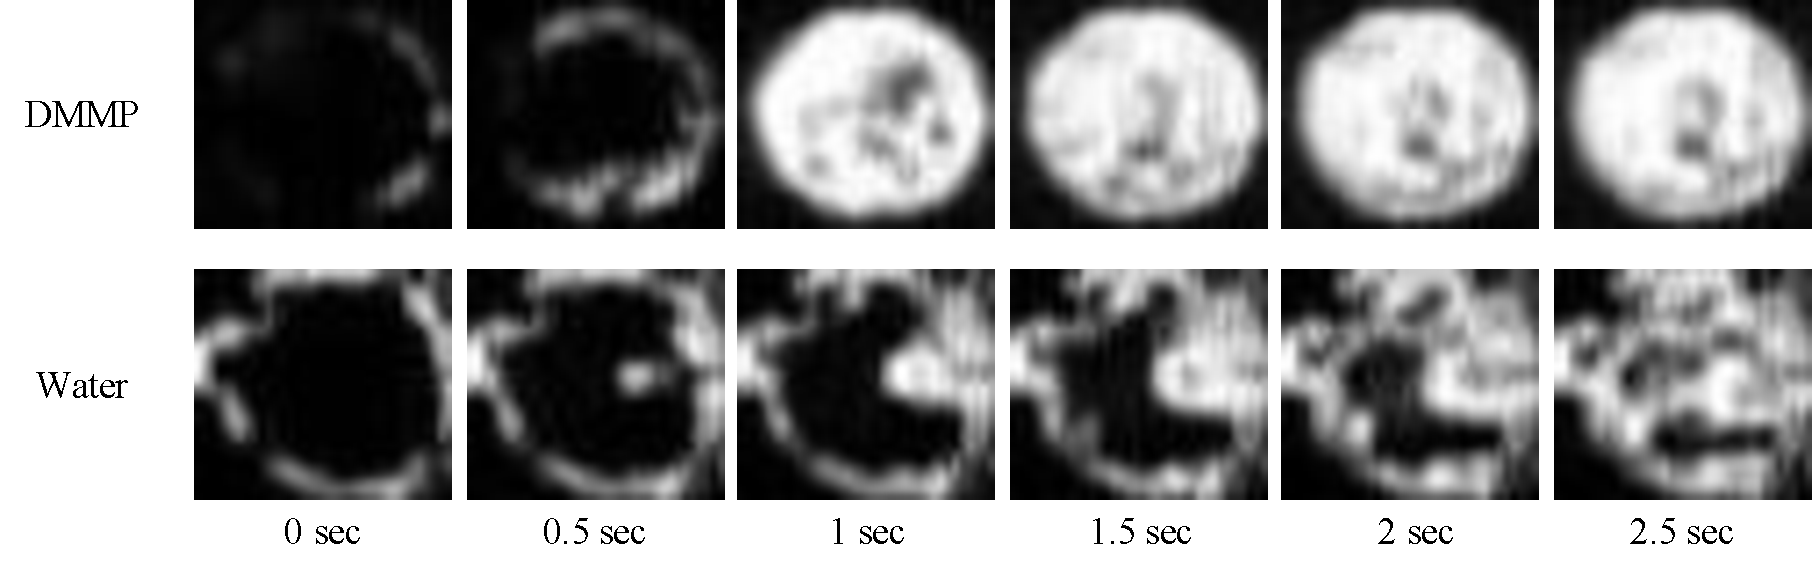
\includegraphics[width=\textwidth]{../fig/lc-raw.pdf}
  \vspace{0.1in}
  \begin{itemize}
  \item DMMP has faster response than water.
    \vspace{0.1in}
  \item The spatial pattern is more uniform in DMMP.
  \end{itemize}
\end{frame}
%------------------------------------------------

%------------------------------------------------
\begin{frame}{Liquid crystal sensor}
  \centering
  \begin{columns}
    \begin{column}{0.35\textwidth}
      \begin{itemize}
      \item Affine model assumed
        \begin{align*}
          \bx^+ = \bA\bx+\bb
        \end{align*}
      \item Rank $2$-solution
        \vspace{0.1in}
      \item A stationary mode and a dynamic mode obtained.
        \vspace{0.1in}
      \item $t_{1/2}=$half life
        \vspace{0.1in}
      \item $T=$period of oscillation.
      \end{itemize}
    \end{column}
    \begin{column}{0.65\textwidth}
  \includegraphics[width=\textwidth]{../fig/lc-main.pdf}
    \end{column}
  \end{columns}
\end{frame}
%------------------------------------------------

%------------------------------------------------
%% \begin{frame}{Outline}
%% \tableofcontents[currentsection]
%% \end{frame}
%------------------------------------------------


%------------------------------------------------
%% \begin{frame}{Electricity market}
%%   \includegraphics[width=\textwidth]{../fig/elec-raw.pdf}
%%   \vspace{0.1in}
%%   \begin{itemize}
%%   \item Can low-rank system ID recover daily, weekely, seasonal flucationations?
%%     \vspace{0.1in}
%%   \item Can we cluster the regions where the price changes coherently?
%%     \vspace{0.1in}
%%   \item Can we construct predictive models with external factors (e.g., weather)?
%%   \end{itemize}
%%   \blfootnote{Image source: Shao et al. (2019)}
%% \end{frame}
%------------------------------------------------

%------------------------------------------------
\begin{frame}{Conclusions}
  \begin{columns}
    \begin{column}{0.6\textwidth}
      \begin{itemize}
      \item We have presented a novel {\blue low-rank system ID} formulation and its closed-form solution, which improves DMD.
        \vspace{0.3in}
        %% \item The identified low-rank model can be used for prediction and predictive control.
        %%   \vspace{0.3in}
      \item The dynamic modes of the low-rank model can be used for characterizing the dynamic behavior of the liquid crystal sensor.
        \vspace{0.3in}
      \item In the future, the technique will be applied to real-time imaging-based control.
      \end{itemize}
    \end{column}
    \begin{column}{0.4\textwidth}
      \includegraphics[width=\textwidth]{../fig/thermal-image.pdf}
    \end{column}
  \end{columns}
\end{frame}
%------------------------------------------------
\begin{frame}
  \titlepage
\end{frame}

\backupbegin
%% ------------------------------------------------
\begin{frame}{Latent variable interpretation}
    \centering
  \begin{tikzpicture}[thick,scale=0.7, every node/.style={transform shape}]
    \fill[black,opacity=0.2] (-2,4) rectangle (2,8);
    \fill[black,opacity=0.2] (4,4) rectangle (8,8);
    \fill[black,opacity=0.2] (1,0) rectangle (5,3);
    \node at (3,2) {$\Big[\tilde{\bx}_i\Big]$};
    \node at (0,6.5) {$\Bigg[\bx_i\Bigg]$};
    \node at (6,6.5) {$\Bigg[\bx_{i+1}\Bigg]$};
    \node at (0,4.5) {Original space $\mathbb{R}^m$};
    \node at (6,4.5) {Original space $\mathbb{R}^m$};
    \node at (3,.5) {Latent space $\mathbb{R}^r$};
    \draw[->] (0.5,6.5) -- (5.5,6.5);
    \draw[->] (0,4) to [out=270,in=180] (2.6,2);
    \draw[->] (3.4,2) to [out=0,in=270] (6,4);
    \draw[->] (6.5,.8) to (6.5,4);
    \draw (3,2.6) -- (3,2.2) (3,1.8) -- (3,1.4);
    \draw (0,7.8) -- (0,6.7) (0,6.3) -- (0,5.2);
    \draw (6,7.8) -- (6,6.7) (6,6.3) -- (6,5.2);
    \node at (3,6.8) {$\bA$};
    \node at (5.3,3) {$\bU$};
    \node at (.7,3) {$\bV^\top$};
    \node at (6.5,.5) {input};
  \end{tikzpicture}
  \begin{itemize}
  \item Dynamics may be explained by a small number of {\em\blue latent variables}
    \vspace{0.1in}
  \item If $\bA=\bU\bV^\top$ with $\bU\in\mathbb{R}^{m\times r}$ and $\bV\in\mathbb{R}^{m\times r}$, then {\blue $\rank(\bA)\leq r$}.
    \vspace{0.1in}
  \item One can always construct latent variable model from the low-rank model
  \end{itemize}
\end{frame}
%------------------------------------------------

%------------------------------------------------
\begin{frame}{Application: predictive control}
  A typical MPC problem can be stated as follows.
  \begin{align*}
    \min_{\bx_k\in\mathbb{X},\bu_k\in\mathbb{U}}\;& \sum_{k=1}^n \ell(\bx_k,\bu_k)\\
    \st\;&\bx^+ = \bA\bx + \bB\bu
  \end{align*}
  If we have a low-rank model  $\bA=\bU\bV^\top$, we can formulate:

  \begin{block}{MPC with low-rank model}
    \vspace{-0.15in}
    \begin{align*}
    \min_{{\blue \tilde{\bx}_k},\bu_k\in\mathbb{U}}\;& \sum_{k=1}^n \ell(\bU{\blue\tilde{\bx}_{k-1}},\bu_k)\\
    \st\;&{\blue\tilde{\bx}^+} = {\blue\tilde{\bA}\tilde{\bx}} + {\blue \tilde{\bB}}\bu \\
    &\bU{\blue\tilde{\bx}_{k-1}}\in\mathbb{X},\;\bu_k\in\mathbb{U}
    \end{align*}
  \end{block}
  \begin{itemize}
  \item $\tilde{\bA}=\bV^\top\bU$, $\tilde{\bB}=\bV^\top\bB$, and $\tilde{\bx}=\bV^\top \bx$
    \vspace{0.1in}
  \item The problem is stated on a {\blue latent variable space}.
    \vspace{0.1in}
  \item The dimension of the problem is reduced.
  \end{itemize}
\end{frame}
%------------------------------------------------
%------------------------------------------------
%% \begin{frame}{Future work}
%%   \begin{block}{Generalized low-rank system ID}
%%     \vspace{-0.1in}
%%     \begin{align*}
%%       \min_{\mathcal{A}\in\mathbb{R}^{p\times m}}\;& \Vert\bY-\mathcal{A}\bX\Vert_F^2 + {\blue f(\mathcal{A})}\\
%%       \st\;&\rank(\mathcal{A})\label{eqn:lrank-con}\leq r\\
%%       &{\blue g(\mathcal{A})\leq 0}.
%%     \end{align*}
%%   \end{block}
%%   \begin{itemize}
%%   \item Prior (regularization) and constraints desired ({\blue grey-box system ID}).
%%     \vspace{0.1in}
%%   \item Closed-form solution not avilable.
%%     \vspace{0.1in}
%%   \item Rank-constraints can be handled by using factorized form $\bA=\bU\bV^\top$.
%%     \vspace{0.1in}
%%   \item Solution algorithms will be explored (alternating minimization, ADMM, etc.).
%%   \end{itemize}
%% \end{frame}
%------------------------------------------------
\backupend
\end{document}
